%!TEX root = ../../master.tex

\subsection*{Experiment 2.1 - Application level}
\subsubsection*{Experiment 2.1.1 - Integration points in a synchronous architecture} 

\noindent ONE BIG FIX \\ 

\noindent \textbf{Setup}\\
The setup used for this scenario consists of a Raspberry Pi cluster, a Macbook Pro (test runner), a network switch, a router and cables in between. FIX (common description somewhere?) \\

\noindent \textbf{The services}\\
The services are Java applications built in Spring Boot and Spring Cloud.
For reproducibility: Github and Docker Hub contains source code and Docker images (tag 0.0.7) with the versions used for testing.

used in the experiment can be found at Github, and the Docker images found at Docker Hub with tag 0.0.7.
\\ 
Tools such as: Hystrix for timeouts, delay and fallbacks \\


\noindent \textbf{Results from the rest of our experiments are presented below} \\

\noindent \textbf{No delay and no circuit breakers with two and three services} \\
The measurements below serve as a reference point before delays are introduced.

\begin{figure}[H]
\centering
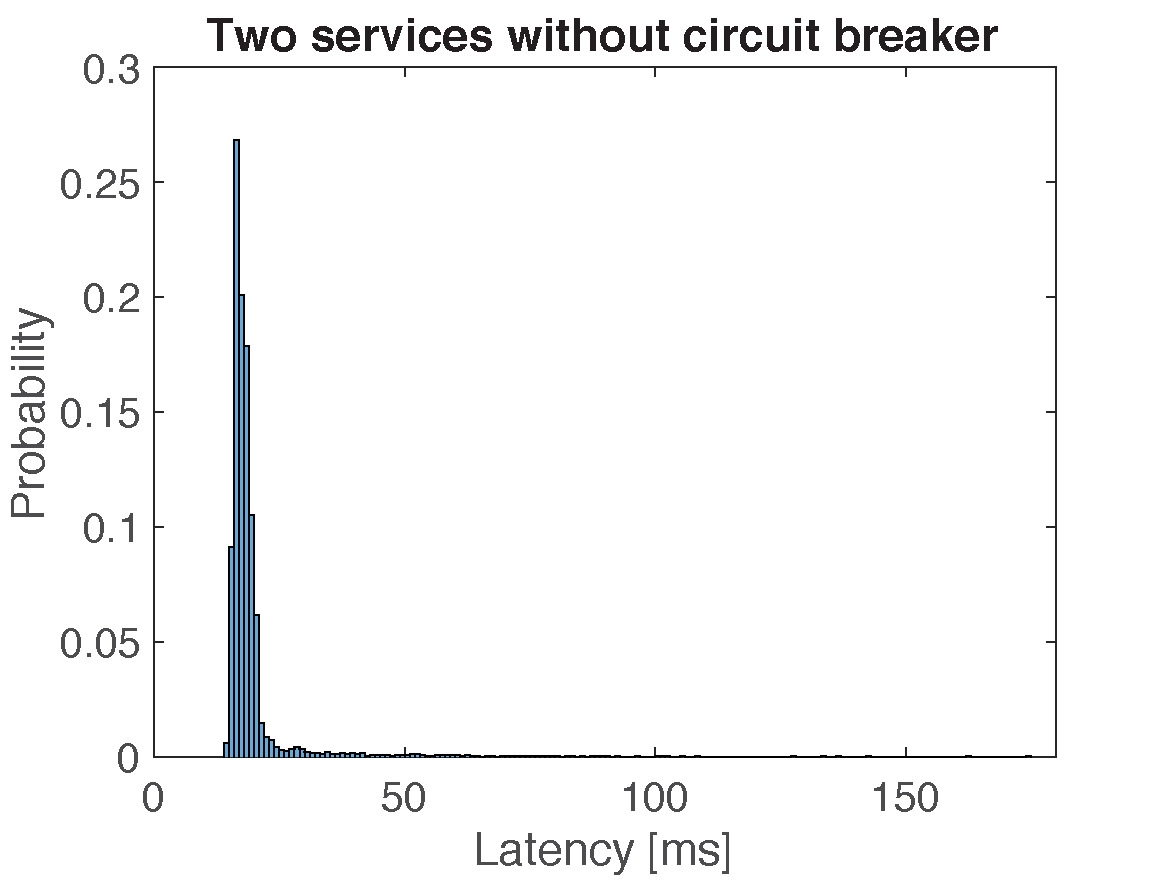
\includegraphics[width=7.5cm]{figures/appendix/nocb_2svc}
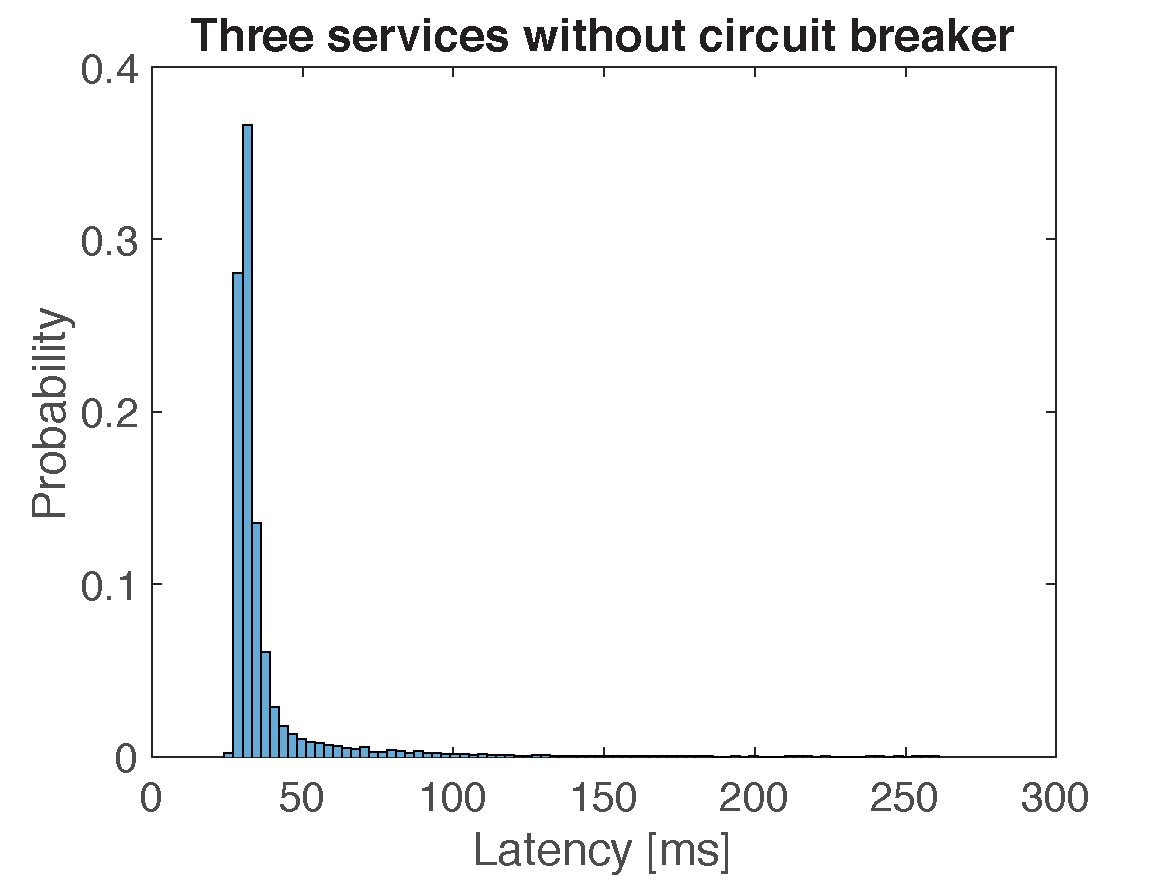
\includegraphics[width=7.5cm]{figures/appendix/nocb_3svc}
\caption{No delay and no circuit breakers}
\label{fig:appendix_circuit_breakers_no_delay}
\end{figure} 


\noindent \textbf{Delay}
\begin{figure}[H]
\centering
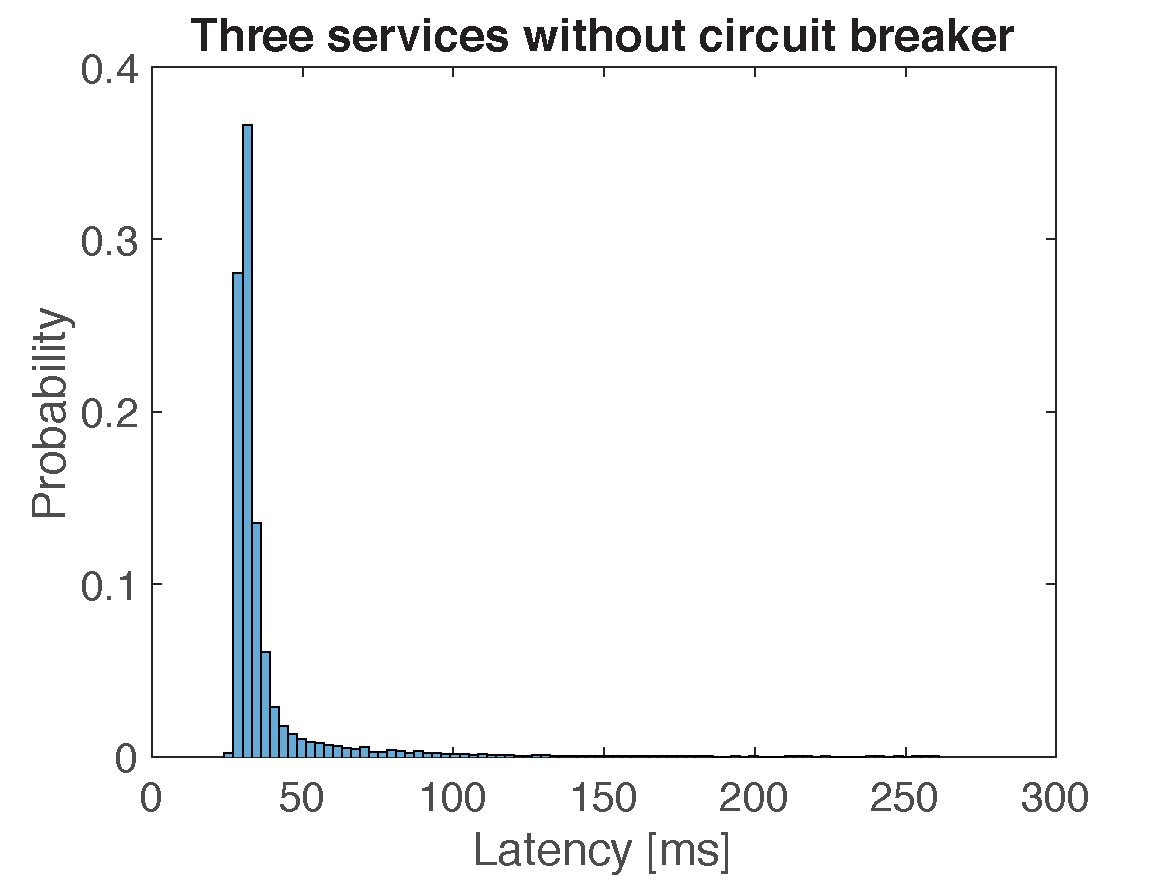
\includegraphics[width=10cm]{figures/appendix/nocb_3svc}
\caption{Delay and no circuit breakers}
%\label{fig:appendix_circuit_breakers_no_delay}
\end{figure} 

\begin{figure}[H]
\centering
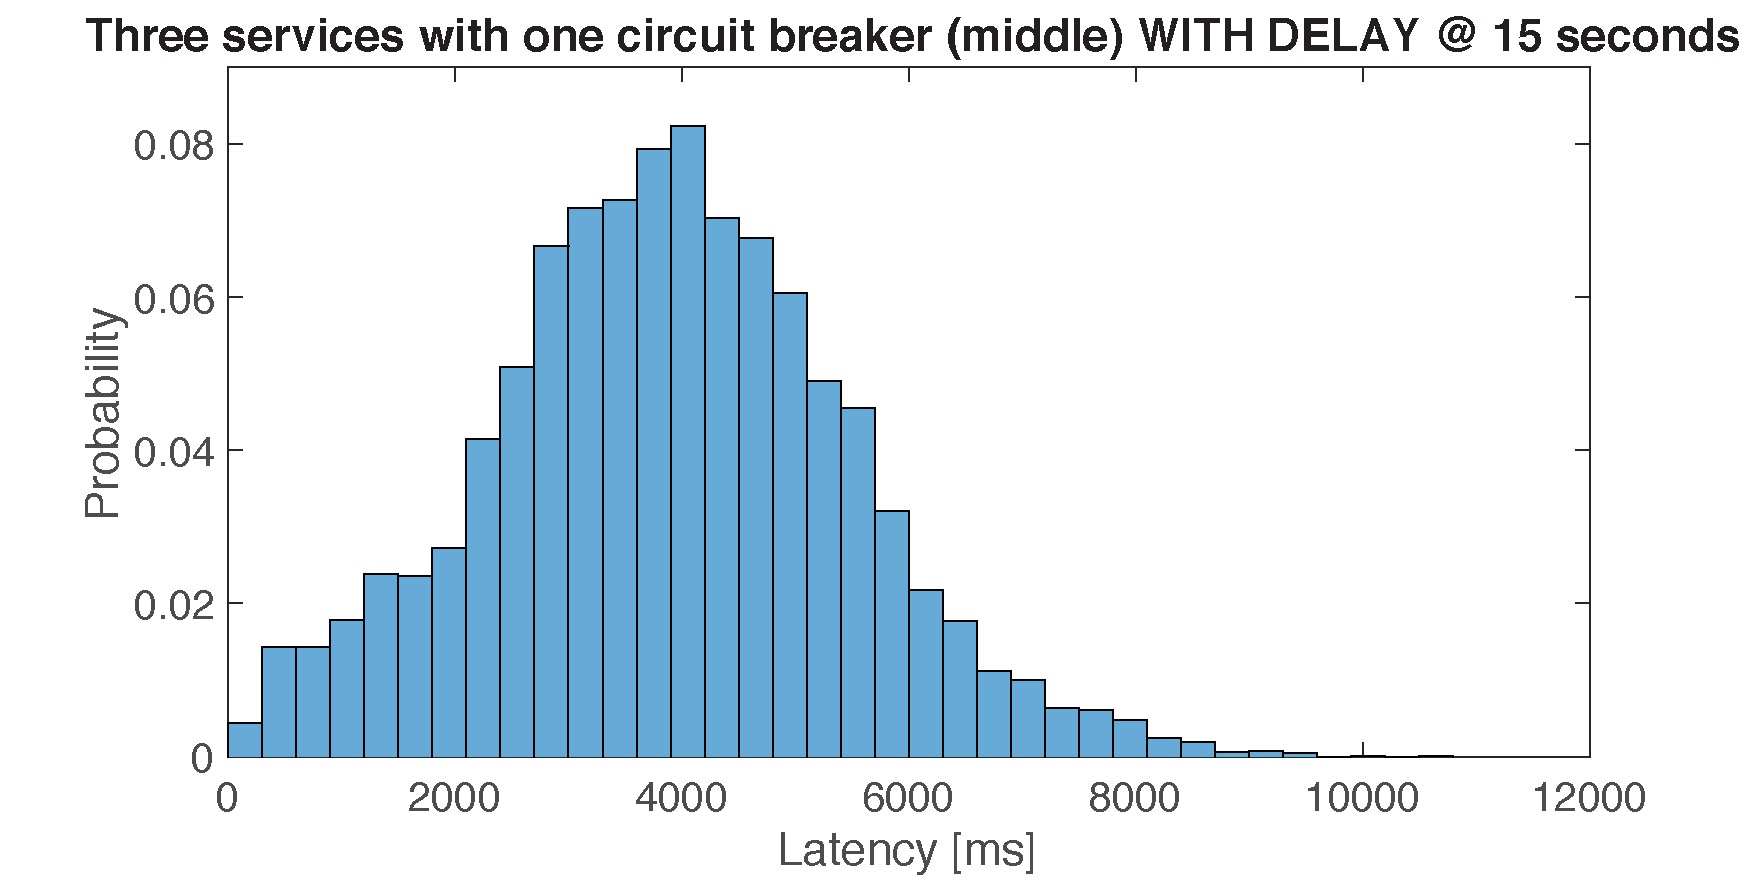
\includegraphics[width=10cm]{figures/appendix/onecb_3svc_delay}
\caption{Delay and one circuit breaker}
%\label{fig:appendix_circuit_breakers_no_delay}
\end{figure} 

\begin{figure}[H]
\centering
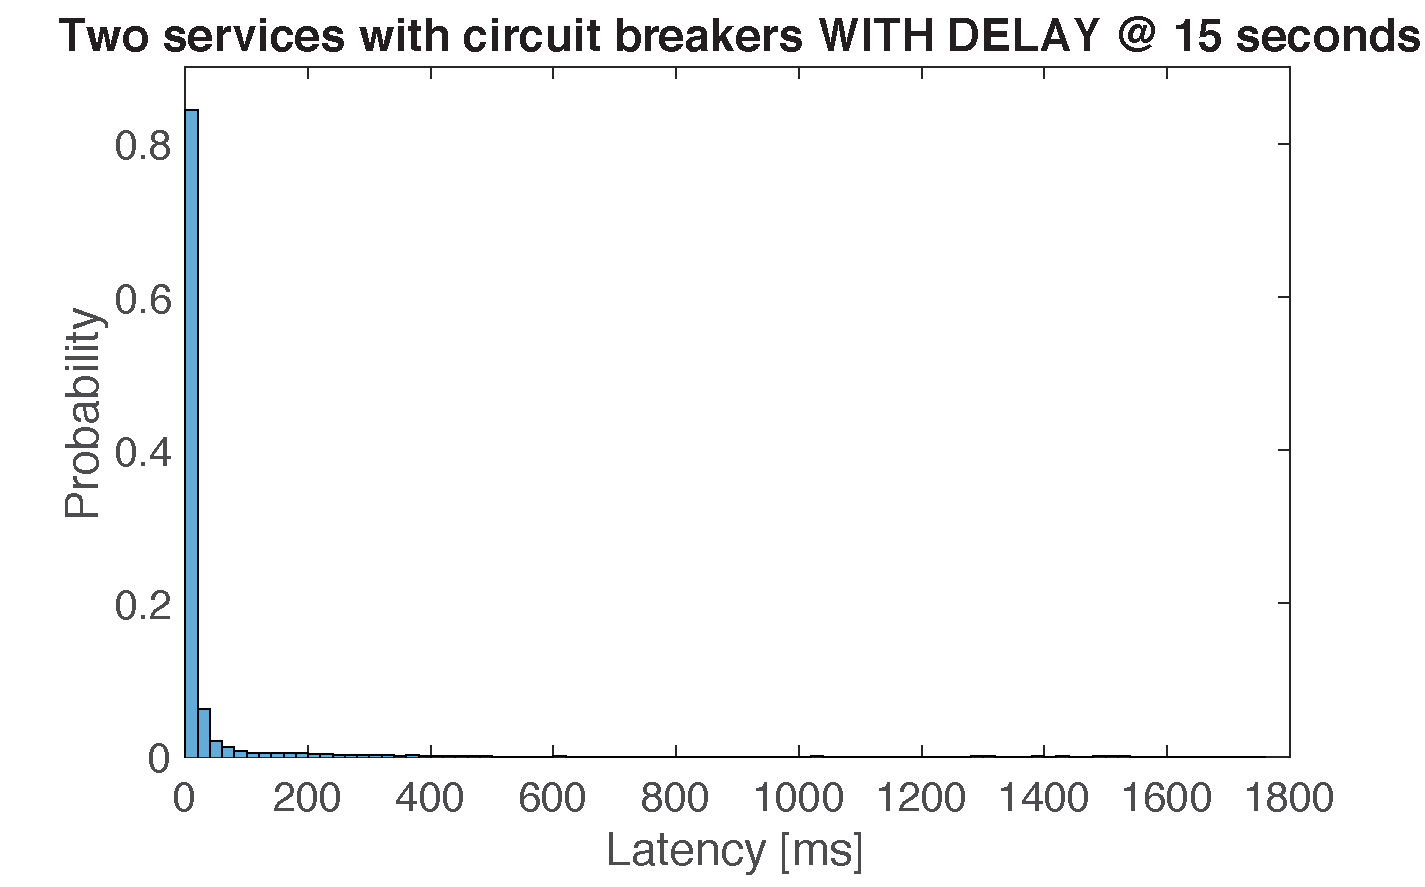
\includegraphics[width=10cm]{figures/appendix/cb_2svc_delay}
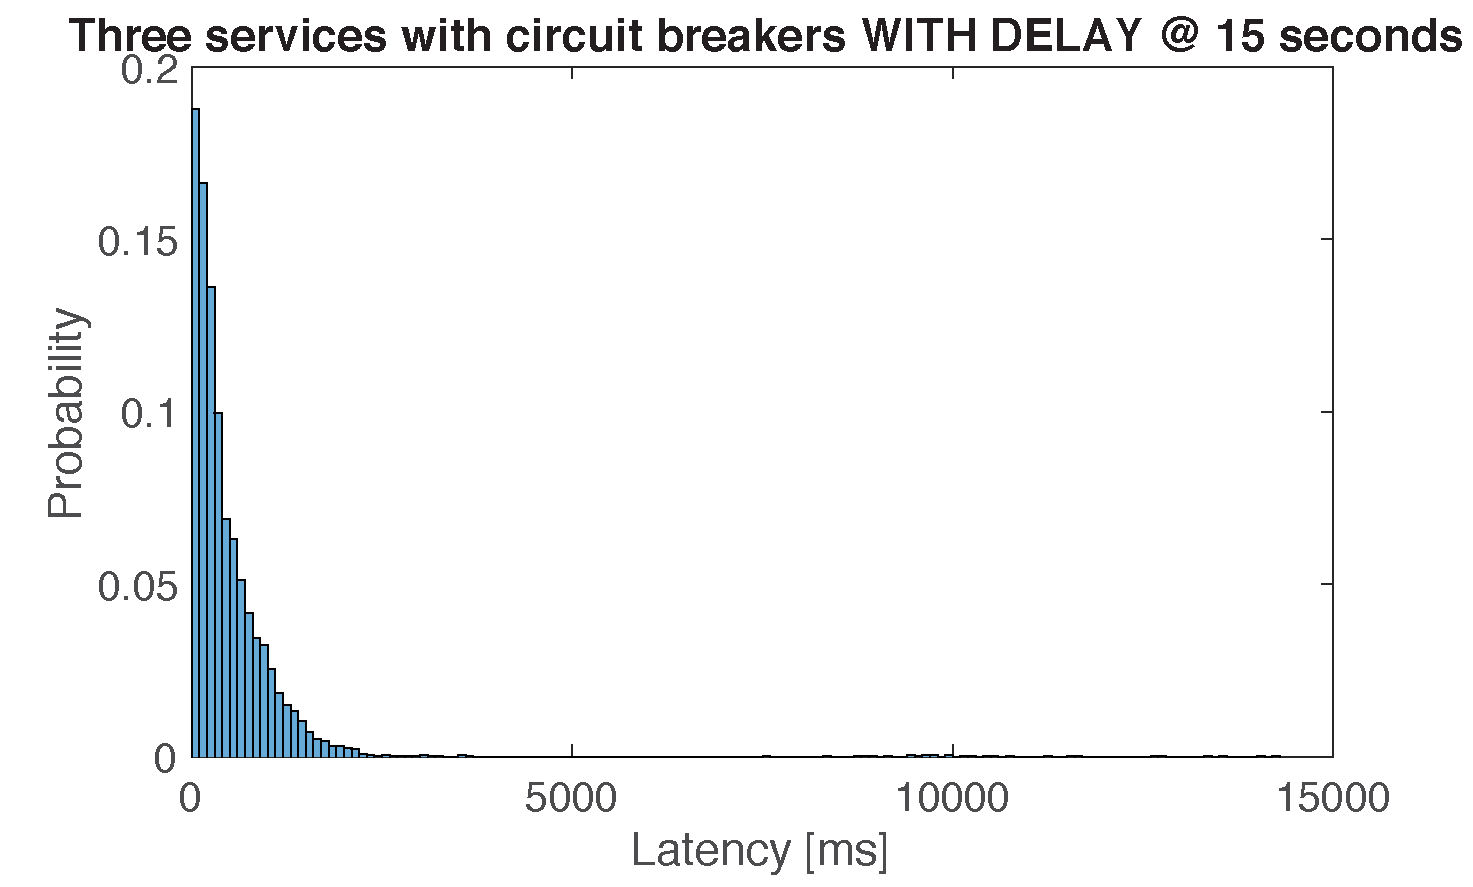
\includegraphics[width=10cm]{figures/appendix/twocb_3svc_delay}
\caption{Delay and circuit breaker(s)}
%\label{fig:appendix_circuit_breakers_no_delay}
\end{figure} 


\noindent \textbf{Individual tables from results section} \\
Split the results from Results into separate columns with each iteration of each scenario. \\

\noindent \textbf{Experiment scripts} \\
Several scripts were used to run these tests. These are presented below.

\noindent
FIX INSERT SCRIPTS \\

\noindent \textbf{Matlab code} \\
REFERENCE MATLAB CODE





